\documentclass{tufte-handout}
\usepackage{mypackagesv3}
\usepackage{tikz, pgfplots, listings, qtree, forest}
\usetikzlibrary{calc,shapes.multipart,chains,arrows}

 %%%%%%%%%%%%%%%%%%%%%%%%%%%%%%%%%%%%%%%%%%%%%%%% neural network driver code

\usepackage{listofitems} % for \readlist to create arrays
\usetikzlibrary{arrows.meta} % for arrow size
\usepackage[outline]{contour} % glow around text
\contourlength{1.4pt}

% COLORS
\usepackage{xcolor}
\colorlet{myred}{red!80!black}
\colorlet{myblue}{blue!80!black}
\colorlet{mygreen}{green!60!black}
\colorlet{myorange}{orange!70!red!60!black}
\colorlet{mydarkred}{red!30!black}
\colorlet{mydarkblue}{blue!40!black}
\colorlet{mydarkgreen}{green!30!black}

% STYLES
\tikzset{
  % redo colours
  >=latex, % for default LaTeX arrow head
  node/.style={thick,circle,draw=myblue,minimum size=22,inner sep=0.5,outer sep=0.6},
  node in/.style={node,green!20!black,draw=mygreen!30!black,fill=mygreen!25},
  node hidden/.style={node,blue!20!black,draw=myblue!30!black,fill=myblue!20},
  node convol/.style={node,orange!20!black,draw=myorange!30!black,fill=myorange!20},
  node out/.style={node,red!20!black,draw=myred!30!black,fill=myred!20},
  connect/.style={thick,mydarkblue}, %,line cap=round
  connect arrow/.style={-{Latex[length=4,width=3.5]},thick,mydarkblue,shorten <=0.5,shorten >=1},
  node 1/.style={node in}, % node styles, numbered for easy mapping with \nstyle
  node 2/.style={node hidden},
  node 3/.style={node out}
}
\def\nstyle{int(\lay<\Nnodlen?min(2,\lay):3)} % map layer number onto 1, 2, or 3



%%%%%%%%%%%%%%%%%%%%%%%%%%%%%%%%%%%%%%%%%%%%%%%%%%%%%%%%%%%%%%%%%%%%%%%%%



\definecolor{light-gray}{gray}{0.95}
\newcommand{\code}[1]{\colorbox{light-gray}{\texttt{#1}}}

%%%%%%%%%%%%%%%%%%%%%%%%%%%%%%%%%%%%%%%%%%%%%%%%%% - listings driver code
% -- Defining colors:
\usepackage[dvipsnames]{xcolor}
\definecolor{codegreen}{rgb}{0,0.6,0}
\definecolor{codegray}{rgb}{0.5,0.5,0.5}
\definecolor{backcolour}{gray}{0.975}
% Definig a custom style:
\lstdefinestyle{mystyle}{
    backgroundcolor=\color{backcolour},
    commentstyle=\color{pinkishpurple},
    keywordstyle=\color{superblue},
    numberstyle=\tiny\color{codegray},
    stringstyle=\color{pinkishpurple},
    basicstyle=\ttfamily\footnotesize\bfseries,
    breakatwhitespace=false,
    breaklines=true,
    captionpos=t,
    keepspaces=true,
    showspaces=false,
    showstringspaces=false,
    showtabs=false,
    tabsize=2
}
% -- Setting up the custom style:
\lstset{style=mystyle}
%%%%%%%%%%%%%%%%%%%%%%%%%%%%%%%%%%%%%%%%%%%%%%%%%%%%%%%%%%%%%%%%%%%%%%%%%%%

% We will externalize the figures
\title{Data Structures and Algorithms}
\begin{document}
\maketitle

\begin{abstract}
This document contains a collection of notes on Data Structures and
Algorithms as taught in ESC190. I assume the reader knows how to code in C and Python and for the most part, topics covered in ESC180 are not explained unless I think I should. There are places where I supplement
the ESC190 notes with my notes on competitive programming, so these
notes do not replace Qilin's or attending lecture (I go to
lecture... right?). Further, Qilin's notes contain more code
examples because I was lazy.

These notes are not self-contained. Perhaps if I have time I will come
back and flush them out, so someone can read it start to
finish. Nevertheless, hopefully this helps someone! \\[2pt]
\end{abstract}

\textbf{\small This document is dedicated to the Zhang Wentao Fan Club \textsuperscript{TM}}

\begin{center}
\begin{marginfigure}
  \centering
  \includegraphics[width=\textwidth]{guerzhoy.jpg}
  \caption{Michael Guerzhoy's Signature}
\end{marginfigure}
\end{center}

\section{The Prerequisites}
\subsection{Runtime Analysis}
We want to compare different algorithms to see which ones perform
``the best''. We can compare algorithms on how much memory they take
up and how fast they run. These types of analysis are called
\textit{space} and \textit{time} complexity respectively. For the
types of algorithms used in this course, space complexity isn't a big concern.

\noindent\textit{\textsc{Time complexity}} is a measure of how fast an algorithm runs.
\begin{marginfigure}
\begin{tikzpicture}[thick]
    \draw[very thin,color=gray] (-0.1,-0.1) grid (3.9,3.9);

  \draw[->] (-0.2,0) -- (4.2,0) node[right] {$x$};
  \draw[->] (0,-0.1) -- (0,4.2) node[above] {$f(x)$};

  \draw[color=orange, domain=0:4]    plot (\x,\x)             node[right] {$O(n)$};
   %\draw[color=blue, domain=1:4]   plot (\x,{ln(\x)/ln(2)}) node[right] {$O(\log n)$};  % Corrected label
   %\draw[color=orange, domain=0:2.7499] plot (\x,{(\x)*ln(\x)/ln(2)}) node[right] {$O(n\log n)$};
  \draw[color=pinkishpurple, domain=0:2] plot (\x,{(\x)*(\x)}) node[right] {$O(n^2)$};
\end{tikzpicture}
  \label{fig:bigoh}
\caption{Example graphs of time complexities.}
\end{marginfigure}
Since different compilers and processors take different amounts
of time to run, it's helpful to look at the number of steps it takes
for a program to run based on input size, and not compilation time.
Specifically, we look at the greatest possible steps it takes for an algorithm to compile \footnote{Re: ESC180. Little explanation given here}\footnote{This is the asymptotic upper bound of compilation steps.}. In other words, we are concerned with the worst possible case of an algorithm which we describe using Big Oh notation: $O(f(n))$, where $n$ represents the number of inputs $f(n)$ represents the number of steps to compile. Figure \ref{fig:bigoh} shows $O(n)$ and $O(n^2)$ time complexities.

Importantly, Big Oh notation only considers the behaviour, or general shape of a function as the input size tends to infinity\footnote{For a more mathematically rigorous treatment of time complexity, check out Donald Knuth's Art of Computer Programming. But to summarize, we can find constants $M$ and $n_0$ so that $O(f(n)) \leq M |f(n)|$ for all $n \geq n_0$ (this just states that $O(f(n))$ has an upper bound)}. So, constant and lower order terms are ignored (think about taking the limit of $f(n)$ as $n$ tends to infinity, only higher order terms are significant). The rules are summarized below. I was too lazy to derive them, but I hope they are at least somewhat intuitive from the idea that big oh notation describes the shape of a function.
\begin{align*}
  f(n) &= O(f(n)) \text{ a function is bounded by itself}\\
  c \cdot O(f(n)) &= O(f(n)) \\
  O(f(n)) + O(f(n)) &= O(f(n)) \\
  O(O(f(n))) &= O(f(n)) \text{ Bounding something that's already bounded does not change the bound}\\
  O(f(n))O(g(n)) &= O(f(n)g(n)) \text{ I don't have a good way of thinking of this yet}
\end{align*}

\textit{You don't need to know the rules above, but they are cool.}

\section{Data Structures}
Data structures help organize and store "structural relations" data\footnote{Relationships between different pieces of data}. Without data structures, data would be stored as amorphous blobs which are hard to keep track of. ESC190 studies linked lists, stacks, queues, priority queues and arrays which are commonly used data structures.
\subsection{Linked Lists}
Linked lists store a data point, and a pointer to the next data point. So suppose you have a list of integers: \code{\{12,99,37,-4,-9,15\}}, then you can visualize a linked list as follows:

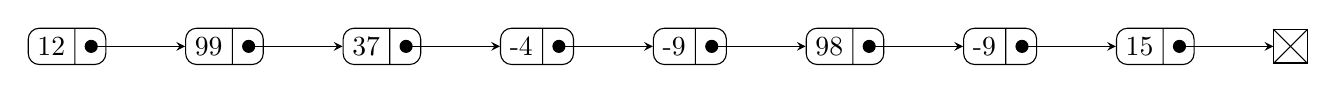
\begin{tikzpicture}[list/.style={rectangle split, rectangle split parts=2,
    draw, rectangle split horizontal, rounded corners}, >=stealth, start chain]

  \node[list,on chain] (A) {12};
  \node[list,on chain] (B) {99};
  \node[list,on chain] (C) {37};
  \node[list,on chain] (D) {-4};
  \node[list,on chain] (E) {-9};
  \node[list,on chain] (F) {98};
  \node[list,on chain] (I) {-9};
  \node[list,on chain] (J) {15};

  \node[on chain,draw,inner sep=6pt] (K) {};
  \draw (K.north east) -- (K.south west);
  \draw (K.north west) -- (K.south east);
  \draw[*->] let \p1 = (A.two), \p2 = (A.center) in (\x1,\y2) -- (B);
  \draw[*->] let \p1 = (B.two), \p2 = (B.center) in (\x1,\y2) -- (C);
  \draw[*->] let \p1 = (C.two), \p2 = (C.center) in (\x1,\y2) -- (D);
  \draw[*->] let \p1 = (D.two), \p2 = (E.center) in (\x1,\y2) -- (E);
  \draw[*->] let \p1 = (E.two), \p2 = (E.center) in (\x1,\y2) -- (F);
  \draw[*->] let \p1 = (F.two), \p2 = (F.center) in (\x1,\y2) -- (I);
  \draw[*->] let \p1 = (I.two), \p2 = (I.center) in (\x1,\y2) -- (J);
  \draw[*->] let \p1 = (J.two), \p2 = (J.center) in (\x1,\y2) -- (K);
\end{tikzpicture}

One way to implement a linked list is to define a \code{node} data
type that contains a data value, and a pointer to the next element in
the linked list. You need to know how to append and delete elements at
some index and search for nodes of specified values in a linked
list. The terminating node always points to
\code{null}\footnote{There's also something called
  \textit{doubly-linked lists} which is linked list where each noted
  stores a pointer to the previous node in addition to a pointer to
  the next node.}. The implementation for linked list is long and is
included in the appendices.

\subsection{Stacks}
Imagine a stack of plates. The last plate you add to the stack is the
first to be taken out of the stack. If you take your plate to be data,
you get a stack data structure!\footnote{This type of data structure
  is called LIFO - last in first out}
\begin{lstlisting}[language=Python]
class Stack:
    def __init__(self):
        self.data = []
    def add(self, val):
        self.data.append(val)
    def pop(self):
        return self.data.pop(val)
\end{lstlisting}
Python lists make the \code{pop} operation very easy.
\subsection{Queues}
Imagine a queue (lineup) of people. The first person to enter the line is the first to leave. Now imagine the people you add/remove from the queue is data. That's your queue data structure!
\begin{lstlisting}[language=Python]
class Queue:
    def __init__(self):
        self.data = []
    def add(self, val):
        self.append(val)
    def remove(self)
        returnVal = self.data[0]
        del self.data[0]
        return returnVal
\end{lstlisting}
Please note I did not test the implementations for \code{Stack} and \code{Queue}
\subsection{Graphs}
Graphs store information about relations between pairs of objects in a collection of objects\footnote{This is hard to understand, fix later}. We can visualize graphs to contain objects called nodes and connections between nodes called edges.
\begin{figure}[ht]
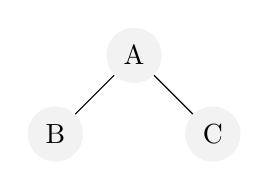
\begin{tikzpicture}[shorten >=1pt,->]
  \tikzstyle{vertex}=[circle,fill=black!5,minimum size=20pt,inner sep=2pt]
  \node[vertex] (G_1) at (-1,-1) {B};
  \node[vertex] (G_2) at (0,0)   {A};
  \node[vertex] (G_3) at (1,-1)  {C};
  \draw (G_1) -- (G_2) -- (G_3) -- cycle;
\end{tikzpicture}
\caption{A simple graph.}
\end{figure}
We can have undirected graphs, where you can move freely between
nodes, and directed graphs, where you move in specified directions. We
can also have weights representing the strength of relationship?
between nodes in weighted graphs.

\subsection{Representing Graphs}
Adjacency lists and adjacency matrices are the standard approaches to
representing graphs. We will represent the following graph in both formats.
\begin{figure}[ht]
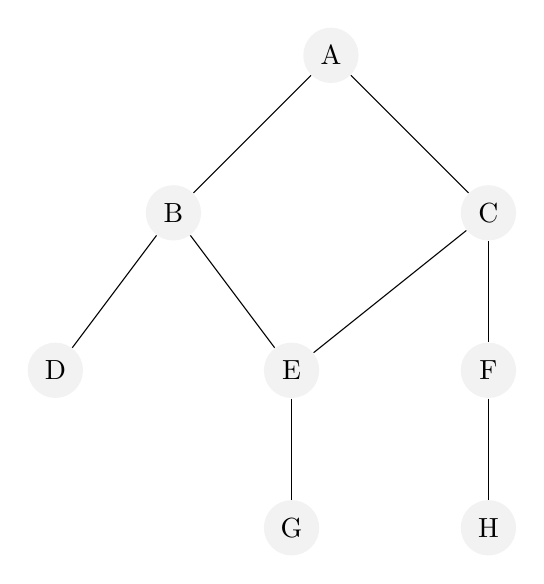
\begin{tikzpicture}[every node/.style={circle, minimum
    size=20pt, inner sep = 2pt,
  fill=black!5}]
  \node (A) at (0,0) {A};
  \node (B) at (-2,-2) {B};
  \node (C) at (2,-2) {C};
  \node (D) at (-3.5,-4) {D};
  \node (E) at (-0.5,-4) {E};
  \node (F) at (2,-4) {F};
  \node (G) at (-0.5,-6) {G};
  \node (H) at (2,-6) {H};

  \draw (A) -- (B);
  \draw (A) -- (C);
  \draw (B) -- (D);
  \draw (B) -- (E);
  \draw (E) -- (G);
  \draw (C) -- (F);
  \draw (F) -- (H);
  \draw (C) -- (E);
\end{tikzpicture}
\caption{Example graph}
\end{figure}

\textbf{Adjacency List:} a list for every node that contains all its neighbours.

\begin{lstlisting}

\end{lstlisting}

% Adjacency Matrix

\section{Dynamic Programming}
\marginpar{\includegraphics[width=\marginparwidth]{exploding-head.png}}
%\begin{marginfigure}[!htbp]
  %\includegraphics[scale=0.01]{exploding-head.png}
%\end{marginfigure}
Dynamic programming (DP) is about reducing repeated computations. This
is done by storing computations, and using them when needed. A classic
example of where DP can be applied is to the recursive implementation
of calculating the fibonacci sequence. Consider the definition of recursive function
\code{fib(n)}:
\begin{lstlisting}[language=Python]
  def fib(n):
    if n == 2:
        return 1

    if n == 1:
        return 0

    else:
        return fib(n-1)+fib(n-2)
\end{lstlisting}
Look for repeated function calls in the call tree for
\code{fib(5)}.
\begin{fullwidth}
\begin{forest}
for tree={
  grow'=south,
  child anchor=north,
  parent anchor=south,
  align=center,
  l sep=12pt,
  s sep=10pt,
  edge={->},
  anchor=center
}
[fib(5)
  [fib(3)
    [fib(1)]
    [fib(2)]
  ]
  [fib(4)
    [fib(2)]
    [fib(3)
      [fib(1)]
      [fib(2)]
    ]
  ]
]
\end{forest}
\end{fullwidth}

\code{fib(3)} and \code{fib{2}} are repeated, for
example. This is a waste of computation resources -
unacceptable. Let's store all our computations, and before making a
new one check if we've done it already. If we have, just use that
value.

\begin{lstlisting}[language=Python]
# just one way to do it!!
n = 5
memo = [-1]*(n+1) # use n+1 to avoid index out of bound error.
# we use -1 to check if memo[n] has been calculated yet.
memo[1], memo[2] = 0, 1

  def fib(n):
    if memo[n] != -1:
        return memo[n]

    if n == 2:
        return memo[2]

    if n == 1:
        return memo[1]

    else:
        memo[n] = fib(n-1)+fib(n-2)
        return memo[n]
\end{lstlisting}

Fun fact: storing recursive function calls is called
\textit{memoization} and storing iterative function calls is called
\textit{tabularization}. For ESC190, you should probably be able to
recognize the DP solution to the coin combination problem.

\section{Graph Theory}
We learned about the graph data structure, and how it can be useful to
represent paths between nodes. A common task is to find a path between
two nodes. We can do this systematically with graph traversal
algorithms. Depth First and Breadth First Search are most common. Play
around with \href{https://visualgo.net/en/dfsbfs?slide=1}{this
  simulation} to visualize different graph traversal
algorithms. You'll notice implementation wise, the only difference
between Breadth First Search and Depth First Search is whether you use
a queue or stack\footnote{To help remember which data structure to use
for BFS or DFS: BFS explores all the neighbours of a node first. So
the first node you see is the first node you explore --> Queue. DFS
explores one path at a time, so all neighbours of a node are explored
later --> Stack.}. 
\subsection{Breadth First Search}
Search along the ``breadth'' of the graph. Again, the algorithm
visualizer linked above is useful to visualize this. Essentially, you
explore all the neighbours of a node at a time. 
\subsection{Depth First Search}
Search along the ``depth'' of a graph. This time, you pick a node, and
explore one path until it terminates\footnote{Good enough reason for
  190}.  
\subsection{Dijkstra's Search}
Dijkstra's search is used when we deal with graphs of with weighted
edges. The weighted edges could represent something like the cost to
make a certain decision (if you think of flowcharts), or maybe the
time of travel to get to a node (if you think nodes as destinations, and
the cost represents how long to travel between destinations).

Our goal is to get from one node to another by taking the lowest
\textit{cost} path, where we define \textit{cost} as the sum of edge weights
between two nodes\footnote{Note to self: terminology can be more
  precise. But hopefully the idea is clear.}.

Dijkstra's search uses a greedy approach\footnote{The greedy approach
  is when you pick the minimum cost choice at every step of your
  algorithm.} to find this minimum cost path between two nodes. To
perform Dijkstra's search:

\begin{enumerate}
\item Pick a start and target node.
\item Set every node to infinity other than the start node.
\item Explore all the neighbours of the starting node. Store
  \code{min(current cost, new cost)} to go to each neigbhour node. Note the cost is cumulative.
  \item Pick the neighbour node with the smallest cost.
  \item Repeat the same type of exploration at the node you picked.
    \item Repeat until you reach the target node.
\end{enumerate}

Qilin Xue posted the pseudocode for Dijkstra's which I'll
include. Some notation: $G=(V,E)$ represents a connected graph $G$
that has interconnected vertices $V$ and edges $E$. The notation $V\S$
refers to the set of vertices that are in $V$ but not in S. $|(u,v)|$
is the weight of the edge connecting $u$ and $v$.

\begin{lstlisting}
Dijkstra(G = (V,E), startNode)
    S = startNode # S is the set of explored nodes
    d(startNode) = 0 # d(v) is the shortest path from startNode to v

    while S != V
        choose v in (V \ S) such that d(u) +|(u,v)| is minimized where u is in S
        Add v to S
        Set d(v) = d(u) + |(u,v)|
# Taken from Qilin's notes
\end{lstlisting}

\textbf{Random thoughts:} \\
\begin{itemize}
\item BFS is just Dijkstra's if all edge weights are equal
\item Use a priority queue to efficiently retrieve the next node to explore
\item Time complexity as written: $\mathcal{O}(|V|^2)$\footnote{$|V|$
    is the size of the graph, or number of vertices}. This is
  because in the worst case
\item Time complexity using a pirority queue
\end{itemize}
if all the node weights are the same, is dijkstras the same as bfs?

- implementation
- time complexity
- pq implementation
- time complexity
-
closing thoughts:
- BFS is just Dijkstra's algorithm if all the edge weights are equal

\color{pinkishpurple}
\subsection{Bonus: Bellman Ford Algorithm}
The Bellman Ford search algorithm is similar to Dijkstra's but handles
graphs with negative weights. This is done by checking for the minimum
cost to each node's neighbours $N-1$ times, where $N$ is the number of
nodes in the graph. The idea is that by $N-1$ iterations, you are
guranteed to have found the minimum distances to every node. It's not
exactly repeating Dijkstra's algorithm multiple
times, and each iteration your graph input is the output of the previous
iteration\footnote{For the first iteration, set all node distances to
infinity}. The difference is that Dijkstra's explores the lowest cost\footnote{You can think of this as the closest neighbouring nodes}
unvisited neighbours to a node; Bellman Ford explores all neighbours.

\begin{lstlisting}
BellmanFord(G = (V,E), startNode)
    # initialize distance to every node to infinity except for the start node
    d() = inf #d(v) is the shortest path from startNode to v
    d(startNode) = 0 # d(v) is the shortest path from startNode to v

    for x in range |G|-1 # |G| is the number of nodes in graph G
        for each edge (u,v) that has weight w
            if distance(u) + w < distance(v)
                Set d(v) = d(u) + w
\end{lstlisting}

The pseudocode does not include an additional step to check for
\textit{negative-weight cycles}. This happens when the cost to take a
path decreases every iteration. For instance, consider the following
graph cycle:

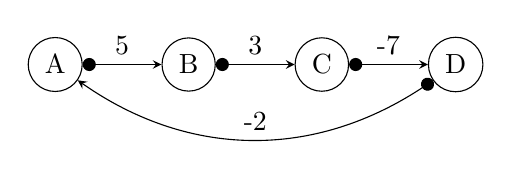
\begin{tikzpicture}[>=stealth, start chain]

  \node[circle, draw, on chain] (A) {A};
  \node[circle, draw, on chain] (B) {B};
  \node[circle, draw, on chain] (C) {C};
  \node[circle, draw, on chain] (D) {D};

  \draw[*->] let \p1 = (A.east), \p2 = (A.center) in
    (\x1,\y2) -- (B) node[midway, above] {5};

  \draw[*->] let \p1 = (B.east), \p2 = (B.center) in
    (\x1,\y2) -- (C) node[midway, above] {3};

  \draw[*->] let \p1 = (C.east), \p2 = (C.center) in
    (\x1,\y2) -- (D) node[midway, above] {-7};

  % Add a curved arrow from D back to A
  \draw[*->, bend left=35] (D) to node[midway, above] {-2} (A);

\end{tikzpicture}

The sum of costs in this cycle is $5+3-7-2=-1$. When the Bellman Ford
algorithm checks the costs of this cycle again (remember it does it
$|V|-1$ times). In this case, the least cost path is undefined. If the
cycle sum is positive, the sum jumps to infinity which is not a
problem, since our goal is to find the least cost path from the
starting node to any other node on the graph. 

So, Dijkstra's takes a greedy approach and Bellman Ford takes a brute
force approach. We can prove we find the optimal solution after $N-1$ iterations.

\subsection{Greedy Best First Search}
Greedy Best First Search is like Dijkstra's except we choose the next
node to explore based on an heuristic function. An heuristic function is something we define for a given
problem that tells us approximately how far away we are from our
goal. We pick the node to explore that has the minimum value in our
heuristic function.

For instance, consider a maze-finding
algorithm. We are at a fork in the maze. Our heurestic function is the
euclidean distance from where we are to the end of the maze. We choose
the path that has the minimium distance to the end of the maze first,
before exploring the longer path. \textbf{Greedy Best First Search
  does not gurantee you find the least path cost between two nodes}
but is \textit{usually} quicker than Dijkstra's since your choice of
node to visit takes you closer to your destination.   

\subsection{A* Search}
A* is like Greedy Best First Search but we incorporate the edge weight
too. See
\href{https://theory.stanford.edu/~amitp/GameProgramming/AStarComparison.html}{this
link} for more information.

\subsection{Binary and Binary Search Trees}


\section{Bonus: An Introduction to Statistical Learning}
\textcolor{pinkishpurple}{\textbf{NOTE:} I'm speedrunning this section and should probably be studying for exams right now. As such, I'm skipping a lot of definitions, explanations, and equation typesetting. A book I like that explains this in depth is \textit{An Introduction to Statistical Learning} by Gareth M. James, Daniela Witten, Trevor Hastie and Robert Tibshirani. }


We collect a lot of data and want to draw conclusions from it. Statistical learning is a branch of mathematics focussed on finding conclusions from data.

The simplest problem involves taking two variables we think are correlated, and trying to find how to get from one variable value to the other. For example, consider a set of observations $X=\{X_1, X_2, X_3,..., X_n\}$ which we may be related to another variable $Y=\{Y_1, Y_2, Y_3, ..., Y_n\}$. We aim to find a function $f$ that maps $X_i \in X$ to $Y_i \in Y$. So, $f(X) = Y$.

Finding $f$ is helpful for \textit{inference} (estimating model parameters)\footnote{this can be explained better} and \textit{prediction} (predicting what $Y$ would be for some $X_k$ that isn't in $X$).

\subsection{Clustering}
Sometimes we have a lot of data that seems to organize itself into distinct groups.



UPDATE FIGURE: change colouring, double check the matrix math stuff
\begin{figure*}
\begin{tikzpicture}[x=2.7cm,y=1.6cm]
  \message{^^JNeural network activation}
  \def\NI{5} % number of nodes in input layers
  \def\NO{4} % number of nodes in output layers
  \def\yshift{0.4} % shift last node for dots

  % INPUT LAYER
  \foreach \i [evaluate={\c=int(\i==\NI); \y=\NI/2-\i-\c*\yshift; \index=(\i<\NI?int(\i):"n");}]
              in {1,...,\NI}{ % loop over nodes
    \node[node in,outer sep=0.6] (NI-\i) at (0,\y) {$a_{\index}^{(0)}$};
  }

  % OUTPUT LAYER
  \foreach \i [evaluate={\c=int(\i==\NO); \y=\NO/2-\i-\c*\yshift; \index=(\i<\NO?int(\i):"m");}]
    in {\NO,...,1}{ % loop over nodes
    \ifnum\i=1 % high-lighted node
      \node[node hidden]
        (NO-\i) at (1,\y) {$a_{\index}^{(1)}$};
      \foreach \j [evaluate={\index=(\j<\NI?int(\j):"n");}] in {1,...,\NI}{ % loop over nodes in previous layer
        \draw[connect,white,line width=1.2] (NI-\j) -- (NO-\i);
        \draw[connect] (NI-\j) -- (NO-\i)
          node[pos=0.50] {\contour{white}{$w_{1,\index}$}};
      }
    \else % other light-colored nodes
      \node[node,blue!20!black!80,draw=pinkishpurple!20,fill=pinkishpurple!5]
        (NO-\i) at (1,\y) {$a_{\index}^{(1)}$};
      \foreach \j in {1,...,\NI}{ % loop over nodes in previous layer
        %\draw[connect,white,line width=1.2] (NI-\j) -- (NO-\i);
        \draw[connect,myblue!20] (NI-\j) -- (NO-\i);
      }
    \fi
  }

  % DOTS
  \path (NI-\NI) --++ (0,1+\yshift) node[midway,scale=1.2] {$\vdots$};
  \path (NO-\NO) --++ (0,1+\yshift) node[midway,scale=1.2] {$\vdots$};

  % EQUATIONS
  \def\agr#1{{\color{mydarkgreen}a_{#1}^{(0)}}} % green a_i^j
  \node[below=16,right=11,mydarkblue,scale=0.95] at (NO-1)
    {$\begin{aligned} %\underset{\text{bias}}{b_1}
       &= \color{mydarkred}\sigma\left( \color{black}
            w_{1,1}\agr{1} + w_{1,2}\agr{2} + \ldots + w_{1,n}\agr{n} + b_1^{(0)}
          \color{mydarkred}\right)\\
       &= \color{mydarkred}\sigma\left( \color{black}
            \sum_{i=1}^{n} w_{1,i}\agr{i} + b_1^{(0)}
           \color{mydarkred}\right)
     \end{aligned}$};
  \node[right,scale=0.9] at (1.3,-1.3)
    {$\begin{aligned}
      {\color{mydarkblue}
      \begin{pmatrix}
        a_{1}^{(1)} \\[0.3em]
        a_{2}^{(1)} \\
        \vdots \\
        a_{m}^{(1)}
      \end{pmatrix}}
      &=
      \color{mydarkred}\sigma\left[ \color{black}
      \begin{pmatrix}
        w_{1,1} & w_{1,2} & \ldots & w_{1,n} \\
        w_{2,1} & w_{2,2} & \ldots & w_{2,n} \\
        \vdots  & \vdots  & \ddots & \vdots  \\
        w_{m,1} & w_{m,2} & \ldots & w_{m,n}
      \end{pmatrix}
      {\color{mydarkgreen}
      \begin{pmatrix}
        a_{1}^{(0)} \\[0.3em]
        a_{2}^{(0)} \\
        \vdots \\
        a_{n}^{(0)}
      \end{pmatrix}}
      +
      \begin{pmatrix}
        b_{1}^{(0)} \\[0.3em]
        b_{2}^{(0)} \\
        \vdots \\
        b_{m}^{(0)}
      \end{pmatrix}
      \color{mydarkred}\right]\\[0.5em]
      {\color{mydarkblue}\mathbf{a}^{(1)}} % vector (bold)
      &= \color{mydarkred}\sigma\left( \color{black}
           \mathbf{W}^{(0)} {\color{mydarkgreen}\mathbf{a}^{(0)}}+\mathbf{b}^{(0)}
         \color{mydarkred}\right)
    \end{aligned}$};

\end{tikzpicture}
\end{figure*}

\appendix
\section{Linked Lists Implementation}
\subsection{Python implementation}
\begin{lstlisting}[language=Python]
class Node:
    def __init__(self, data):
        self.data = data
        self.next = None # points to null by default
class LL():
    def __init__(self):
        # store head node
        self.head = None

    def get_i(self, i):
        x = 0
        cur = self.head
        while x < i:
            cur = cur.next
            x += 1
        return cur.data

    def append(self, value):
        # traverse to end of linkedlist and add a node
        newNode = Node(value) # create new node
        # case 1: head node is None
        if self.head == None:
            self.head = newNode

        else:
            # find the last node
            cur = self.head
            while cur.next != None:
                cur = cur.next
            cur.next = newNode
    def insert(self, value, i):
        newNode = Node(value)
        if i == 0:
            tmp = self.head
            self.head = newNode
            newNode.next = tmp # this can be done in two lines by the way
        else:
            cur = self.head
            for i in range (i-1):
                cur = cur.next
            newNode.next = cur.next
            cur.next = newNode
    def printLL(self):
        cur = self.head
        if cur == None:
            print("empty")
        while (cur != None):
            print(cur.data, " ", end="")
            cur = cur.next

# driver code
hi = LL()
hi.append(4)
hi.append(5)
print("hello")
hi.printLL()
print("\n")
hi.insert(5,2)
hi.printLL()
print(hi.get_i(2))
\end{lstlisting}
\subsection{C implementation}

\end{document}
%%% Local Variables:
%%% mode: latex
%%% TeX-master: t
%%% End:
